\documentclass[11pt,a4paper]{article}

\usepackage[margin=2.5cm]{geometry}
\usepackage{amsmath,amssymb}
\usepackage{booktabs,array,tabularx}
\usepackage{graphicx}
\usepackage[font=small,labelfont=bf]{caption}
\usepackage{pdflscape}
\usepackage{float}
\usepackage[authoryear,round]{natbib}
\usepackage{enumitem}
\usepackage{setspace}
\usepackage{xcolor}
\usepackage[colorlinks=true,linkcolor=blue!50!black,citecolor=blue!50!black,urlcolor=blue!50!black]{hyperref}

\graphicspath{{../figures/}}
\setstretch{1.15}
\setlist{itemsep=2pt,topsep=4pt}

\newcommand{\En}{\mathbb{E}_n}
\newcommand{\E}{\mathbb{E}}
\newcommand{\Rnuis}{\hat R_{\mathrm{nuis}}}
\newcommand{\code}[1]{\texttt{#1}}

\title{\textbf{Nuisance Function Structure and Finite-Sample Inference\\ in Double Machine Learning}\\[0.4em]
\large A Comparison of Additive Splines and Neural Networks in the Partially Linear Model}
\author{Jiankun Wang\\ ECON472 Senior Honours Essay}
\date{November 2026}

\begin{document}
\maketitle

\begin{abstract}
\noindent This essay asks whether the match between the true nuisance functions and the learner explains the finite-sample coverage of double machine learning (DML) confidence intervals in the partially linear model. A Monte Carlo experiment with known nuisance functions crosses an additive and an interactive design with two sample sizes (500, 2000) and two ambient dimensions (10, 50). Linear regression, an additive cubic spline with a ridge penalty and a two-layer ReLU network serve as first-stage learners in the DoubleML partialling-out estimator with 5-fold cross-fitting. Each replication records the first-stage errors on an independent test sample and an exact decomposition of the estimation error into a sampling term, cross terms and a second-order term. With 50 replications per cell, three results emerge. First, the bias is the second-order term: their correlation across cells is 0.998, and coverage predicted from that term alone is within 0.03 of the observed rate on average. Second, structural match decides the size of that term. The spline covers 88--92\% of the time in the additive design (except at $n=500$, $p=50$) but 14--16\% in the interactive design at $n=2000$; the network is the only learner near nominal in the interactive design (88\% at $n=2000$, $p=10$) and is beaten by the spline in the additive design. Third, learners whose error stalls at their approximation limit give intervals that get worse as $n$ grows. The exact second-order term predicts coverage far better than the usual upper-bound proxy (rank correlation $-0.97$ against $-0.78$), because the proxy cannot distinguish systematic misfit from estimation noise. Dropping cross-fitting did not raise the network's bias, because the resulting cross terms happened to offset the second-order term. In an application to 401(k) eligibility, the spline and the network agree on an effect of about \$9,000 on net financial assets, while linear regression gives \$5,900; the same decomposition attributes most of the gap to an income misfit shared by both nuisance functions.

\medskip
\noindent\textbf{Keywords:} double machine learning; partially linear model; Neyman orthogonality; neural networks; additive splines; cross-fitting; Monte Carlo.
\end{abstract}

% =====================================================================
\section{Introduction}

Double machine learning lets researchers control for many covariates with flexible prediction methods and still report a standard confidence interval for a treatment effect. The guarantee behind that interval is conditional: the first-stage prediction errors must be small enough that their product vanishes faster than $n^{-1/2}$. Whether a particular learner meets this condition, at a particular sample size, for a particular data generating process, is an empirical question. Applied work rarely checks it.

This essay asks one question. \emph{In the partially linear model, does the structural match between the nuisance functions and the learner explain the finite-sample coverage of DML confidence intervals, through its effect on out-of-sample prediction error and on the second-order remainder?} The proposal broke this into four testable hypotheses:
\begin{itemize}
\item[\textbf{H1.}] Coverage falls as the second-order remainder grows.
\item[\textbf{H2.}] When the nuisance functions are smooth and additive, additive splines do no worse than a small neural network, in first-stage error and in coverage.
\item[\textbf{H3.}] When the functions have low effective dimension but contain interactions or composite indices, the neural network attains a smaller first-stage error and may achieve better coverage.
\item[\textbf{H4.}] For complex learners in difficult designs, cross-fitting gives smaller bias or more stable coverage than fitting without sample splitting.
\end{itemize}

The evidence comes from a Monte Carlo experiment with known nuisance functions. Two designs, one additive and one interactive, are crossed with two sample sizes (500, 2000) and two ambient dimensions (10, 50). Each sample is analysed with linear regression, an additive cubic spline with a ridge penalty, and a two-layer ReLU network, all within the DoubleML partialling-out estimator with 5-fold cross-fitting. Because the truth is known, every replication records the first-stage errors on an independent test sample and the exact decomposition of the estimation error into a sampling term, cross terms and a second-order term.

Three findings stand out.
\begin{enumerate}
\item \textbf{The bias is the second-order term.} Across all learner-design cells the Monte Carlo bias and the mean second-order term have a correlation of 0.998. A normal approximation that uses only this term predicts coverage to within 0.03 on average. The standard error is accurate throughout; failed intervals are displaced, not too narrow.
\item \textbf{Structural match decides the size of that term.} Additive splines reach 0.88--0.92 coverage in the additive design (except at $n=500$, $p=50$) but fall to 0.14--0.16 in the interactive design at $n=2000$, because their error there stalls at the additive approximation limit. The network is the only learner near nominal in the interactive design (0.88 at $n=2000$, $p=10$), and it is beaten by the spline in the additive design.
\item \textbf{More data can make intervals worse.} A learner stuck at a fixed approximation error has a constant bias while the standard error shrinks, so coverage falls with $n$. Linear regression covers 56--60\% of the time at $n=500$ in the interactive design but 0--4\% at $n=2000$.
\end{enumerate}

The essay adds to the literature in a deliberately modest way. It does not prove new rates. Instead it turns the product-rate condition of DML theory into a quantity that can be measured in each replication, and shows that the exact second-order term explains coverage far better than both the learner's name and the usual upper-bound proxy for the remainder (rank correlation with coverage $-0.97$ against $-0.78$).

Section~\ref{sec:lit} reviews the related literature. Section~\ref{sec:model} sets out the model, the orthogonal score and the error decomposition. Section~\ref{sec:design} describes the Monte Carlo design and Section~\ref{sec:results} the results. Section~\ref{sec:app} applies the three learners to the effect of 401(k) eligibility on net financial assets. Section~\ref{sec:disc} discusses mechanisms, limitations and practical guidance, and Section~\ref{sec:concl} concludes. Appendix~\ref{app:walk} works through one replication by hand.

% =====================================================================
\section{Related literature}\label{sec:lit}

This essay connects three strands of work: semiparametric estimation in the partially linear model, the double/debiased machine learning (DML) framework, and the approximation theory of nonparametric learners.

\paragraph{Partially linear models and orthogonality.} \citet{robinson1988} showed that the coefficient on $D$ in the partially linear model can be estimated at the root-$n$ rate by ``partialling out'' $X$ from both $Y$ and $D$ with kernel regressions. \citet{newey1994} characterised the asymptotic variance of such semiparametric estimators and the role of the first-stage estimator in it. The idea of a moment condition that is locally insensitive to the nuisance parameter goes back to \citet{neyman1959}. \citet{chen2014} derive the semiparametric efficiency bound in partially linear single-index models, which is the natural benchmark when the nuisance function is itself low-dimensional.

\paragraph{Double machine learning.} \citet{belloni2014} used orthogonal moments with Lasso-selected controls to obtain valid inference after model selection. \citet{chernozhukov2018} generalised the approach: a Neyman-orthogonal score combined with cross-fitting delivers root-$n$ consistent, asymptotically normal estimates of the target parameter whenever the product of the nuisance estimation errors is $o_p(n^{-1/2})$. Because the condition is stated in terms of prediction errors, it is learner-agnostic. The DoubleML package \citep{bach2022,bach2024} implements the framework and is used here for all estimation.

\paragraph{What determines first-stage error.} For isotropic $s$-smooth functions of $p$ variables the minimax $L_2$ rate is $n^{-s/(2s+p)}$ \citep{stone1982}, which deteriorates quickly with $p$. Additive models escape this curse when the truth is additive: each component is estimated at a one-dimensional rate \citep{stone1985,hastie1990}. Deep ReLU networks attain rates governed by the effective dimension of a compositional structure rather than by $p$ \citep{schmidthieber2020}, and \citet{farrell2021} show that such rates are fast enough for second-stage semiparametric inference.

\paragraph{Gap addressed here.} These results are sufficient conditions on rates; they do not say whether a given learner, at a given $n$, will be accurate enough for valid confidence intervals. Most applied comparisons of learners report only bias, RMSE and coverage of the final estimate. This essay instead measures the first-stage errors against known true functions and computes the exact second-order term of the DML estimator in every replication. That makes it possible to trace a coverage failure back through the remainder to the mismatch between the learner and the true function.

% =====================================================================
\section{Model and estimator}\label{sec:model}

The DML estimate differs from the truth by a mean-zero sampling term plus a second-order term equal to the product of the two first-stage errors. This section derives that decomposition exactly, because the Monte Carlo evidence in Section~\ref{sec:results} is organised around it.

\subsection{The partially linear model}

Let $W=(Y,D,X)$, with outcome $Y$, scalar treatment $D$ and covariates $X\in\mathbb{R}^p$:
\begin{align}
Y &= \theta_0 D + g_0(X) + U, \qquad \E[U\mid D,X]=0, \label{eq:y}\\
D &= m_0(X) + V, \qquad \E[V\mid X]=0. \label{eq:d}
\end{align}
The nuisance functions $g_0$ and $m_0$ are unknown. Define $\ell_0(X)=\E[Y\mid X]=\theta_0 m_0(X)+g_0(X)$. Subtracting conditional means gives $Y-\ell_0(X)=\theta_0\{D-m_0(X)\}+U$, so whenever $\E[V^2]>0$,
\[
\theta_0=\frac{\E\big[(D-m_0(X))(Y-\ell_0(X))\big]}{\E\big[(D-m_0(X))^2\big]}.
\]

\subsection{The Neyman-orthogonal score}

The estimator solves the sample analogue of $\E[\psi(W;\theta_0,\eta_0)]=0$ for the partialling-out score
\begin{equation}\label{eq:score}
\psi(W;\theta,\eta)=\big\{Y-\ell(X)-\theta\,(D-m(X))\big\}\big\{D-m(X)\big\},\qquad \eta=(\ell,m).
\end{equation}
The score is Neyman orthogonal: its expectation does not move, to first order, when the nuisance functions are perturbed away from the truth. To see this, let $\Delta\ell=\ell-\ell_0$ and $\Delta m=m-m_0$ and evaluate the score along the path $\eta_0+r(\eta-\eta_0)$:
\[
\E\,\psi(W;\theta_0,\eta_0+r\Delta)=\E\big[\{U-r(\Delta\ell-\theta_0\Delta m)\}\{V-r\Delta m\}\big]=r^2\,\E\big[\Delta m\,(\Delta\ell-\theta_0\Delta m)\big].
\]
The three terms that are linear in $r$ vanish: $\E[UV]=0$, $\E[U\,\Delta m(X)]=0$ because $\E[U\mid D,X]=0$, and $\E[V f(X)]=0$ for any $f$ because $\E[V\mid X]=0$. The derivative at $r=0$ is therefore zero, and only a product of the two errors survives. By contrast, the naive plug-in score $(Y-\theta D-g(X))D$ gives $\E=-r\,\E[\Delta g(X)\,m_0(X)]$, which is first order in the error. With a naive score, a first-stage error of order $n^{-1/4}$ produces a bias of the same order, far larger than the $n^{-1/2}$ standard error.

Figure~\ref{fig:orth} shows the difference numerically. On one sample of 1,000,000 draws from DGP~A, both nuisance functions are pushed away from the truth along the shape a linear learner misses ($X_2^2-1$), and $\theta$ is re-estimated with each score. The orthogonal score's bias grows with the square of the error (log-log slope 1.99), the naive score's linearly (slope 1.00). At an error of 10\% of the maximum perturbation, the orthogonal bias is 0.0018 and the naive bias $-0.0153$.

\begin{figure}[t]
\centering
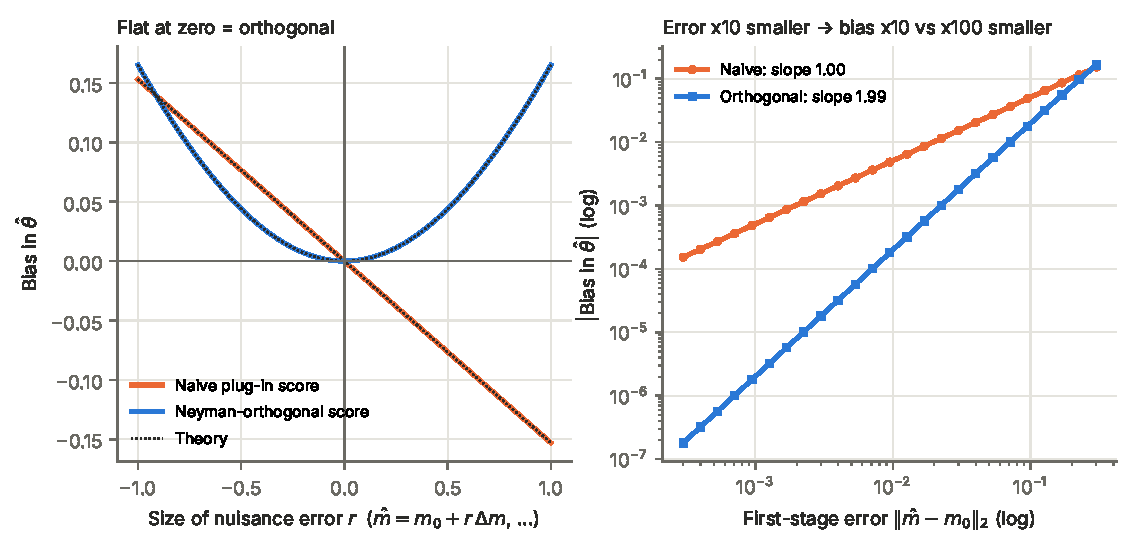
\includegraphics[width=\textwidth]{fig6_orthogonality_demo.pdf}
\caption{Bias of $\hat\theta$ under the orthogonal and a naive plug-in score as the nuisance error grows (left), and on log scales (right).}\label{fig:orth}
\end{figure}

\subsection{Cross-fitting and the standard error}

The sample is split into $K=5$ folds. For each fold $k$, $\ell$ and $m$ are fitted on the other four folds and used to predict the held-out observations, giving residuals $\tilde Y_i=Y_i-\hat\ell^{(-k)}(X_i)$ and $\tilde D_i=D_i-\hat m^{(-k)}(X_i)$. Pooling the residuals across folds (the DML2 estimator),
\[
\hat\theta=\frac{\sum_i\tilde D_i\tilde Y_i}{\sum_i\tilde D_i^2},\qquad
\hat J=\frac1n\sum_i\tilde D_i^2,\qquad
\hat\sigma^2=\frac{\frac1n\sum_i(\tilde Y_i-\hat\theta\tilde D_i)^2\tilde D_i^2}{\hat J^2},\qquad
\mathrm{SE}=\hat\sigma/\sqrt n.
\]
The 95\% interval is $\hat\theta\pm1.96\cdot\mathrm{SE}$. Cross-fitting ensures that each observation's residual comes from a model that never saw it, so overfitting cannot correlate the first-stage error with that observation's own noise.

\subsection{An exact decomposition of the estimation error}\label{sec:decomp}

Write the out-of-fold errors as $a=m_0-\hat m$ and $b=\ell_0-\hat\ell$. Then $\tilde D=V+a$ and $\tilde Y-\theta_0\tilde D=U+(b-\theta_0a)$. Substituting into $\hat\theta-\theta_0=\En[\tilde D(\tilde Y-\theta_0\tilde D)]/\hat J$ yields an algebraic identity that holds in every sample:
\begin{equation}\label{eq:decomp}
\hat\theta-\theta_0=\underbrace{\frac{\En[VU]}{\hat J}}_{\text{oracle term}}+\underbrace{\frac{\En[aU]+\En[V(b-\theta_0a)]}{\hat J}}_{\text{cross terms}}+\underbrace{\frac{\En[a\,(b-\theta_0a)]}{\hat J}}_{\text{second-order term }\hat R_2}.
\end{equation}
\begin{itemize}
\item The \textbf{oracle term} is what the estimator would be with the true nuisances. It has mean zero, is of order $n^{-1/2}$, and drives the sampling variance.
\item The \textbf{cross terms} are first order in the errors but have mean zero, because cross-fitting makes $(a,b)$ independent of the held-out $(U,V)$. Orthogonality removes the population first-order bias; cross-fitting removes the finite-sample correlation that overfitting would create.
\item The \textbf{second-order term} $\hat R_2$ has non-zero mean and is the bias. Since $\ell=\theta m+g$, $b-\theta_0a$ equals $g_0-\hat g$ with $\hat g=\hat\ell-\theta_0\hat m$, so $\hat R_2$ is the covariance between the error in predicting $D$ and the implied error in $g$.
\end{itemize}

\paragraph{The decomposition is the score's expansion along the path.} Evaluate the sample score at $\theta_0$ along the path from the true nuisances to the fitted ones, $\eta_0+r(\hat\eta-\eta_0)$. Because the score is a product of two residuals that are each linear in $r$, its sample mean is exactly quadratic in $r$:
\begin{equation}\tag{4$'$}\label{eq:path}
\En\,\psi\big(W;\theta_0,\eta_0+r(\hat\eta-\eta_0)\big)=\En[VU]+r\,\big\{\En[aU]+\En[V(b-\theta_0a)]\big\}+r^2\,\En[a(b-\theta_0a)].
\end{equation}
At $r=1$ the left side is $\En[\tilde D(\tilde Y-\theta_0\tilde D)]$, so dividing by $\hat J$ returns \eqref{eq:decomp} term by term. The oracle term is the zero-order coefficient. The cross terms are the first-order coefficient, the sample counterpart of the derivative that orthogonality sets to zero in the population. The second-order term is the curvature. Appendix~\ref{app:walk} evaluates \eqref{eq:path} on one replication.

By Cauchy--Schwarz, $|\hat R_2|\le\|a\|\cdot\|b-\theta_0a\|/\hat J$. Asymptotic normality at the root-$n$ rate therefore requires the familiar product-rate condition
\begin{equation}\label{eq:rate}
\|\hat m-m_0\|_2\big(\|\hat m-m_0\|_2+\|\hat\ell-\ell_0\|_2\big)=o_p\big(n^{-1/2}\big),
\end{equation}
which motivates the proposal's remainder proxy, computed from test-sample errors:
\begin{equation}\label{eq:rnuis}
\Rnuis=\sqrt n\,\|\hat m-m_0\|_2\big(\|\hat m-m_0\|_2+\|\hat\ell-\ell_0\|_2\big).
\end{equation}
The proxy is an upper bound. It is tight when $a$ and $b-\theta_0a$ point in the same direction, as they do when a learner misses the same feature of both functions. It is loose when the errors are mostly estimation noise, which averages out in the product.

\paragraph{From bias to coverage.} If $\hat\theta$ is approximately normal with mean $\theta_0+R_2$ and standard deviation $\sigma/\sqrt n$, and SE estimates $\sigma/\sqrt n$ well, the coverage of the nominal 95\% interval is approximately
\begin{equation}\label{eq:cov}
\text{coverage}\approx\Phi\big(1.96-\sqrt n\,R_2/\sigma\big)+\Phi\big(-1.96-\sqrt n\,R_2/\sigma\big).
\end{equation}
Coverage thus depends only on the standardised bias $\sqrt n\,R_2/\sigma$. A learner whose error stalls at a fixed approximation error has a constant $R_2$, so its standardised bias grows like $\sqrt n$: \textbf{more data makes its intervals less reliable.}

% =====================================================================
\section{Monte Carlo design}\label{sec:design}

The experiment crosses two nuisance structures with two sample sizes and two ambient dimensions, and fits each sample with three learners plus an oracle that uses the true functions.

\subsection{Data generating processes}

In every design $X\sim N(0,\Sigma)$ with $\Sigma_{jk}=0.5^{|j-k|}$, $V$ and $U$ are independent $N(0,1)$, $D=m_0(X)+V$, $Y=\theta_0D+g_0(X)+U$, and $\theta_0=0.5$. Only $X_1$ to $X_4$ enter $m_0$ and $g_0$; raising $p$ from 10 to 50 adds irrelevant covariates without changing the true functions.

\paragraph{DGP A (smooth additive).} Every component is a function of a single covariate, so the truth lies inside the additive class:
\begin{align}
m_0(X)&=0.5\sin(X_1)+0.25(X_2^2-1)+0.25X_3+0.20\tanh(X_4),\label{eq:mA}\\
g_0(X)&=\sin(X_1)+0.50(X_2^2-1)+0.50X_3+0.30\tanh(X_4).\label{eq:gA}
\end{align}

\paragraph{DGP B (low effective dimension, interactive and composite).} The functions depend on the product $X_1X_2$ and the index $X_3+X_4$, which no sum of one-dimensional functions can represent exactly:
\begin{align}
m_0(X)&=0.5\tanh(X_1X_2)+0.25\tanh(X_3+X_4),\label{eq:mB}\\
g_0(X)&=\sin(X_1X_2)+0.50\{\tanh(X_3+X_4)\}^2.\label{eq:gB}
\end{align}

Table~\ref{tab:dgp} reports population diagnostics computed on 200,000 draws. Two features matter for what follows. First, in DGP~A the two nuisance functions are almost collinear (correlation 0.999, $g_0\approx2m_0$), so any feature a learner misses appears with the same sign in both errors. Second, DGP~B has a weaker signal: $X$ explains 9\% of the variance of $D$, against 28\% in DGP~A.

\begin{table}[t]
\centering\small
\caption{Signal strength and best attainable fit of each model class (population values).}\label{tab:dgp}
\begin{tabular}{lcc}
\toprule
Quantity & DGP A & DGP B\\
\midrule
$R^2$ of $D$ on $X$ (share of $\mathrm{Var}\,D$ explained by $m_0$) & 0.281 & 0.087\\
$R^2$ of $Y$ on $X$ (share of $\mathrm{Var}\,Y$ explained by $\ell_0$) & 0.654 & 0.239\\
$\mathrm{Corr}(m_0,g_0)$ & 0.999 & 0.601\\
Share of $\mathrm{Var}\,m_0$ a linear fit can capture & 0.642 & 0.337\\
Share of $\mathrm{Var}\,m_0$ an additive fit can capture & 1.000 & 0.584\\
Share of $\mathrm{Var}\,\ell_0$ an additive fit can capture & 1.000 & 0.240\\
$L_2$ approximation error of best linear fit, $m_0$ / $\ell_0$ & 0.375 / 0.935 & 0.251 / 0.618\\
$L_2$ approximation error of best additive fit, $m_0$ / $\ell_0$ & 0.002 / 0.004 & 0.199 / 0.544\\
\bottomrule
\end{tabular}
\end{table}

The last two rows are floors: no amount of data takes a learner's error below the approximation error of its model class. Plugging them into \eqref{eq:rnuis} gives the remainder proxy that a learner would have even with infinite training data. For the additive class in DGP~B this floor is 3.3 at $n=500$ and 6.6 at $n=2000$; for the linear class in DGP~A it is 11.0 and 22.0.

\subsection{Grid and replications}

The core grid is $n\in\{500,2000\}\times p\in\{10,50\}\times\text{DGP}\in\{A,B\}$, eight points in total. The results below use $R=50$ replications per point, the pilot size in the proposal. With 50 replications, the Monte Carlo standard error of a coverage rate is about 0.03 near 0.95 and 0.07 near 0.50, so differences smaller than about 0.15 are not interpreted. Within a replication, all learners use the same simulated sample and the same five folds (common random numbers), so learner comparisons are paired.

\subsection{Learners}

The same learner class estimates $\ell$ and $m$. All preprocessing and tuning happen inside each training fold, so no information from the held-out fold leaks into the first stage.

\begin{table}[h]
\centering\small
\caption*{Learners and tuning (all tuning inside the training folds).}
\begin{tabularx}{\textwidth}{>{\raggedright\arraybackslash}p{2.6cm}>{\raggedright\arraybackslash}X>{\raggedright\arraybackslash}p{4.2cm}}
\toprule
Learner & Specification & Tuning\\
\midrule
Linear regression & OLS on standardised covariates & none\\
Additive spline & Cubic B-spline basis per covariate, 6 interior knots at quantiles, linear extrapolation, no interactions, ridge penalty & penalty from $\{0.01,0.1,1,10,100\}$ by leave-one-out CV\\
ReLU network & Two hidden layers of 32 units, Adam, learning rate 0.001, early stopping on a 20\% validation split (patience 25, at most 500 epochs), standardised inputs and target & L2 penalty $\alpha$ from $\{1,3,10,30,100\}$ by 3-fold CV\\
Oracle & True $\ell_0$ and $m_0$ & none\\
\bottomrule
\end{tabularx}
\end{table}

The network's penalty grid departs from the proposal's original values. In scikit-learn the L2 term is $(\alpha/2B)\|W\|^2$ per mini-batch of $B=200$ observations, so values of 0.01 or less leave the network effectively unregularised. A preliminary check, run before the pilot, showed that such networks fit noise in the weak-signal DGP~B and predict worse than a constant. A sweep over $\alpha$ from 0.1 to 1000 (Appendix~\ref{app:alpha}) puts the optimum between 3 and 30 in every design, and a finer grid does not improve on the one used. The learning rate was fixed rather than tuned to halve the run time.

\subsection{Metrics}

For each grid point and learner the experiment records the bias, standard deviation and RMSE of $\hat\theta$; the coverage of the 95\% interval and its Monte Carlo standard error; the ratio of the mean SE to the Monte Carlo standard deviation; the mean interval length; and the median test-sample errors $\|\hat m-m_0\|$ and $\|\hat\ell-\ell_0\|$. These errors are computed on an independent sample of 20,000 covariate draws (fixed across replications), averaged over the five fold models. Each replication also stores the three terms of decomposition \eqref{eq:decomp}, the Cauchy--Schwarz bound, and $\Rnuis$ from \eqref{eq:rnuis}. A check that the three terms sum to $\hat\theta-\theta_0$ holds to machine precision in every replication. Appendix~\ref{app:walk} carries out every step of this computation by hand for two replications and checks each number against DoubleML and against the stored simulation output.

\subsection{Software and reproducibility}

All code is in Python 3.13 with NumPy 2.5, pandas 3.0, scikit-learn 1.9 \citep{pedregosa2011} and DoubleML 0.11 \citep{bach2022}. Every seed, grid and hyperparameter is set in one configuration file. Replication seeds are derived from a master seed with NumPy's \code{SeedSequence}, keyed by DGP, $n$ and $p$, so adding a grid point never changes the draws at another. Appendix~\ref{app:code} maps each step to the code.

% =====================================================================
\section{Results}\label{sec:results}

Whether the 95\% interval covers $\theta_0$ is decided almost entirely by the second-order term. In turn, that term is large whenever a learner's model class cannot represent the true nuisance functions at the given sample size. All results use $R=50$ replications per cell.

\subsection{The oracle benchmark and the standard error}

With the true nuisance functions, coverage lies between 0.92 and 0.98 in all eight designs and the bias never exceeds 0.005 in absolute value (Appendix~\ref{app:full}). The ratio of the mean SE to the Monte Carlo standard deviation of $\hat\theta$ is between 0.87 and 1.19 for the oracle. For the three learners it is between 0.83 and 1.22, including every cell where coverage falls below 50\%. The standard error is therefore not the problem: when intervals fail, they have roughly the right width but sit in the wrong place.

\subsection{Coverage by learner}

\begin{table}[t]
\centering\small
\caption{Coverage of the nominal 95\% interval, with the standardised bias (bias / sd of $\hat\theta$) in parentheses. $R=50$; the Monte Carlo standard error of a coverage near 0.5 is about 0.07.}\label{tab:cov}
\begin{tabular}{cccllll}
\toprule
DGP & $n$ & $p$ & Oracle & Linear & Spline & Network\\
\midrule
A & 500 & 10 & 0.98 ($+0.1$) & 0.00 ($+5.0$) & 0.90 ($+0.5$) & 0.60 ($+1.6$)\\
A & 500 & 50 & 0.96 ($-0.1$) & 0.02 ($+3.9$) & 0.28 ($+2.0$) & 0.02 ($+3.6$)\\
A & 2000 & 10 & 0.92 ($+0.0$) & 0.00 ($+7.4$) & 0.92 ($+0.2$) & 0.64 ($+1.4$)\\
A & 2000 & 50 & 0.94 ($-0.1$) & 0.00 ($+8.2$) & 0.88 ($+0.2$) & 0.02 ($+3.6$)\\
B & 500 & 10 & 0.98 ($-0.1$) & 0.56 ($+1.8$) & 0.72 ($+1.5$) & 0.82 ($+1.3$)\\
B & 500 & 50 & 0.92 ($-0.0$) & 0.60 ($+1.5$) & 0.70 ($+1.6$) & 0.72 ($+1.4$)\\
B & 2000 & 10 & 0.98 ($+0.2$) & 0.00 ($+4.5$) & 0.14 ($+3.7$) & 0.88 ($+1.1$)\\
B & 2000 & 50 & 0.96 ($+0.0$) & 0.04 ($+3.9$) & 0.16 ($+3.1$) & 0.12 ($+3.5$)\\
\bottomrule
\end{tabular}
\end{table}

\begin{figure}[t]
\centering
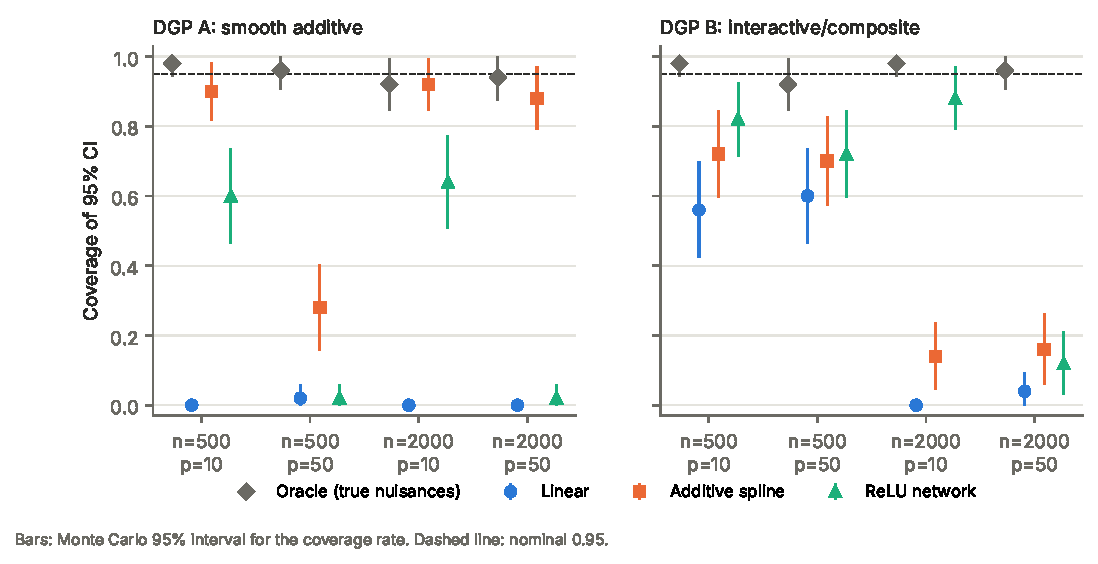
\includegraphics[width=\textwidth]{fig1_coverage.pdf}
\caption{Coverage by learner, DGP, $n$ and $p$. Bars are Monte Carlo 95\% intervals; the dashed line is the nominal level.}\label{fig:cov}
\end{figure}

\textbf{Linear regression} fails in almost every design (Table~\ref{tab:cov}, Figure~\ref{fig:cov}). In DGP~A its bias is 0.23--0.26, about half of $\theta_0$, and coverage is 0.00--0.02. In DGP~B the bias is smaller, 0.084--0.091, and coverage is 0.56--0.60 at $n=500$ but 0.00--0.04 at $n=2000$. The bias does not change with $n$, while the standard deviation halves, so the standardised bias doubles. The apparent partial success at $n=500$ is the wide interval hiding the bias, not the learner working.

\textbf{The additive spline} attains 0.88--0.92 coverage in DGP~A, except at $n=500$, $p=50$, where coverage is 0.28 and the bias is 0.117. In DGP~B it behaves like the linear benchmark: a constant bias of about 0.074 gives coverage of 0.70--0.72 at $n=500$ and 0.14--0.16 at $n=2000$.

\textbf{The ReLU network} reaches 0.88 in DGP~B at $n=2000$, $p=10$, the only learner close to nominal in DGP~B at the larger sample size. Elsewhere it does less well: 0.60--0.64 in DGP~A with $p=10$, and 0.02--0.12 with $p=50$ in DGP~A and in DGP~B at $n=2000$.

\subsection{First-stage errors}

\begin{table}[t]
\centering\small
\caption{Median test-sample errors $\|\hat m-m_0\|$ / $\|\hat\ell-\ell_0\|$ and the mean remainder proxy $\Rnuis$ from \eqref{eq:rnuis}.}\label{tab:err}
\begin{tabular}{ccclll}
\toprule
DGP & $n$ & $p$ & Linear & Spline & Network\\
\midrule
A & 500 & 10 & 0.42 / 0.97 / 13.0 & 0.32 / 0.45 / 5.5 & 0.42 / 0.66 / 10.4\\
A & 500 & 50 & 0.56 / 1.09 / 20.5 & 0.47 / 0.85 / 13.9 & 0.61 / 1.15 / 24.2\\
A & 2000 & 10 & 0.38 / 0.94 / 22.9 & 0.18 / 0.23 / 3.3 & 0.23 / 0.40 / 6.4\\
A & 2000 & 50 & 0.42 / 0.97 / 26.4 & 0.34 / 0.47 / 12.4 & 0.36 / 0.63 / 15.8\\
B & 500 & 10 & 0.30 / 0.66 / 6.7 & 0.28 / 0.61 / 5.6 & 0.32 / 0.64 / 6.8\\
B & 500 & 50 & 0.47 / 0.78 / 13.2 & 0.31 / 0.63 / 6.4 & 0.36 / 0.66 / 8.8\\
B & 2000 & 10 & 0.27 / 0.63 / 10.7 & 0.23 / 0.58 / 8.5 & 0.21 / 0.40 / 5.8\\
B & 2000 & 50 & 0.31 / 0.66 / 13.7 & 0.28 / 0.61 / 10.9 & 0.28 / 0.63 / 11.7\\
\bottomrule
\end{tabular}
\end{table}

\begin{figure}[t]
\centering
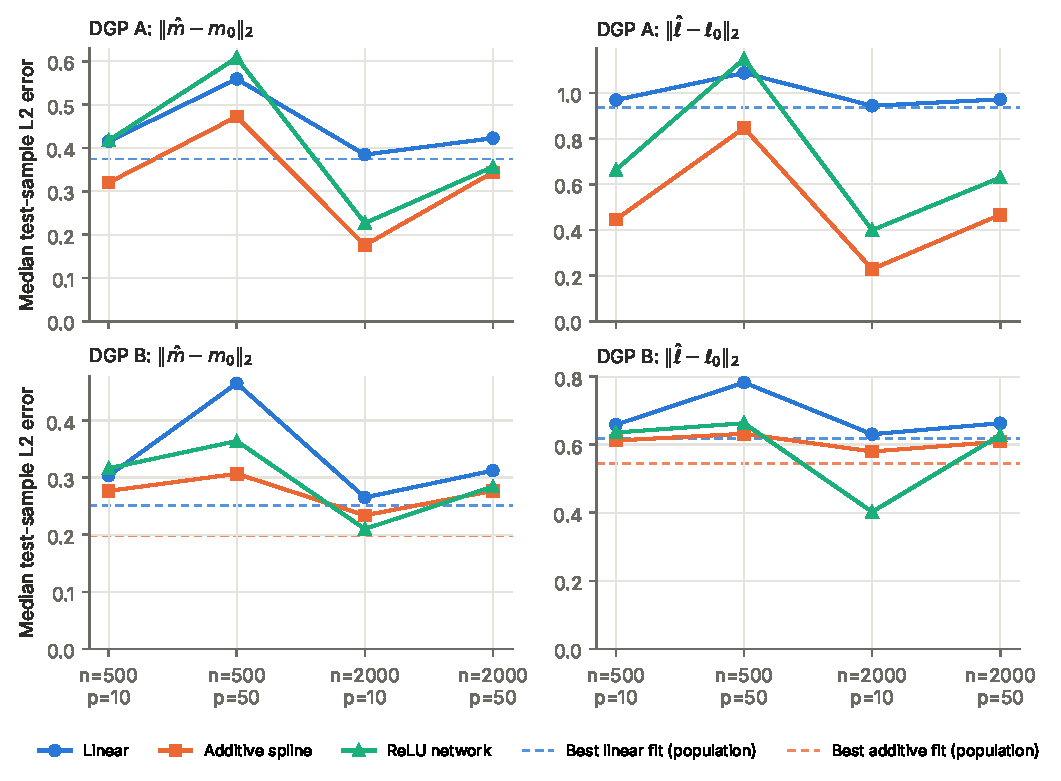
\includegraphics[width=\textwidth]{fig2_nuisance_error.pdf}
\caption{Median test-sample errors of the three learners across the grid. Dashed lines mark the error of the best linear and best additive fit in the population (Table~\ref{tab:dgp}).}\label{fig:err}
\end{figure}

The errors explain the coverage pattern through the approximation floors of Table~\ref{tab:dgp} (Table~\ref{tab:err}, Figure~\ref{fig:err}).
\begin{itemize}
\item \textbf{Linear regression sits on its floor.} Its error for $\ell$ is 0.94--1.09 in DGP~A against a floor of 0.935, and 0.63--0.78 in DGP~B against 0.618. More data cannot reduce it.
\item \textbf{In DGP~A the spline has the lowest error in every cell}, and its error falls with $n$ ($\ell$: from 0.45 to 0.23 at $p=10$) because the truth is additive. At $n=2000$, $p=10$ its errors are 0.18 / 0.23, against 0.23 / 0.40 for the network.
\item \textbf{In DGP~B the spline stalls near its floor.} Its error for $\ell$ stays at 0.58--0.63, close to the additive floor of 0.544. Only the network, at $n=2000$ and $p=10$, goes below that floor, to 0.40. This is the cell where it covers.
\item \textbf{Irrelevant covariates are costly at $n=500$.} At $p=50$ the spline uses about 400 basis functions with 400 training observations, and its error for $\ell$ in DGP~A rises from 0.45 to 0.85. The network's error rises from 0.66 to 1.15, worse than linear regression. An L2 penalty shrinks all weights alike and does not select variables.
\end{itemize}

\subsection{The second-order term explains coverage}

\begin{figure}[t]
\centering
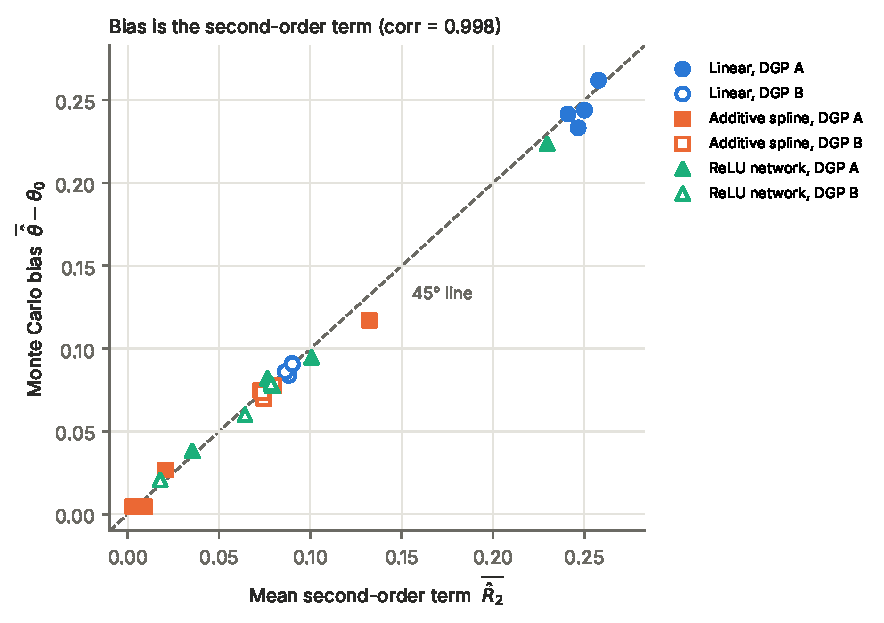
\includegraphics[width=0.78\textwidth]{fig4_bias_vs_second_order.pdf}
\caption{Monte Carlo bias against the mean second-order term $\hat R_2$, by learner and DGP. The dashed line is the 45-degree line.}\label{fig:bias}
\end{figure}

\begin{figure}[t]
\centering
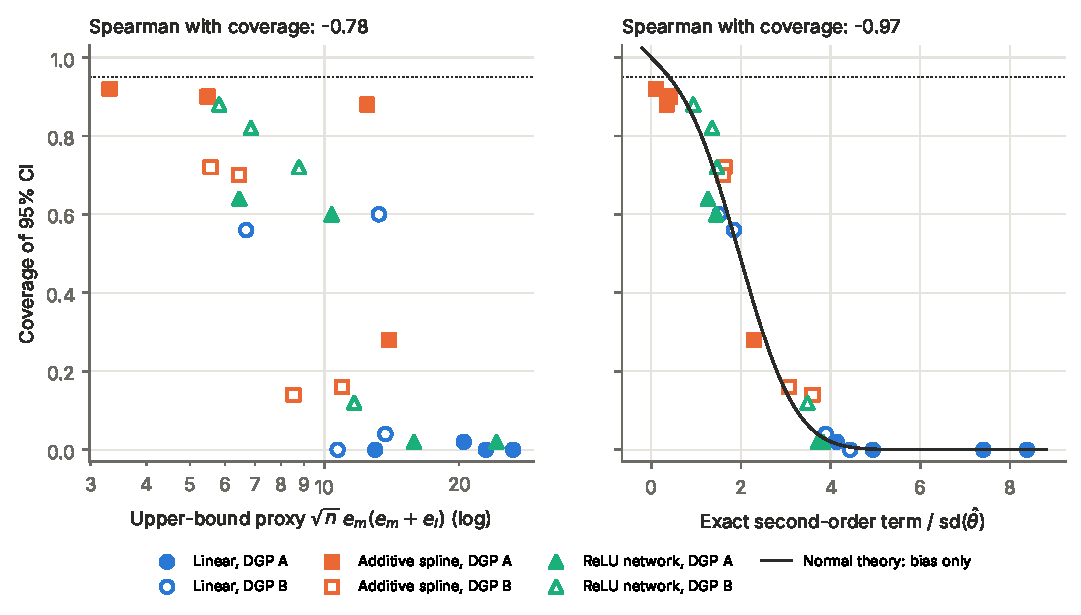
\includegraphics[width=\textwidth]{fig5_coverage_two_proxies.pdf}
\caption{Coverage against the upper-bound proxy $\Rnuis$ (left, log scale) and against the exact second-order term in units of $\mathrm{sd}(\hat\theta)$ (right). The curve is the normal-theory coverage \eqref{eq:cov} implied by the bias alone.}\label{fig:proxies}
\end{figure}

H1 is supported, and the exact term supports it more sharply than the proxy. Across the 24 learner cells:
\begin{itemize}
\item the correlation between the Monte Carlo bias and the mean second-order term is \textbf{0.998} (Figure~\ref{fig:bias});
\item coverage predicted from \eqref{eq:cov}, using only the mean second-order term, the mean SE and $\mathrm{sd}(\hat\theta)$, differs from observed coverage by \textbf{0.030} on average, within Monte Carlo error;
\item the rank correlation of coverage with $|\hat R_2|/\mathrm{sd}(\hat\theta)$ is \textbf{$-0.97$}, against \textbf{$-0.78$} with $\Rnuis$ (Figure~\ref{fig:proxies}).
\end{itemize}

The proxy fails where the first-stage error is mostly estimation noise. The spline in DGP~A at $n=2000$, $p=50$ has $\Rnuis=12.4$, a value that elsewhere goes with coverage below 0.3. Yet its second-order term is only 0.35 standard deviations and coverage is 0.88. Noise in $\hat m$ and in $\hat g$ points in unrelated directions and averages out in the product; misspecification does not.

\begin{table}[t]
\centering\small
\caption{Decomposition \eqref{eq:decomp} of the bias, averaged over the four cells of each DGP. The oracle and cross terms are recorded for replications 21--50 only; the second-order term for all 50.}\label{tab:decomp}
\begin{tabular}{llrrrrr}
\toprule
Learner & DGP & Bias & Oracle term & Cross terms & Second-order term & C--S bound\\
\midrule
Linear & A & 0.245 & 0.001 & $-0.004$ & 0.249 & 0.300\\
Linear & B & 0.088 & 0.001 & $-0.001$ & 0.089 & 0.177\\
Spline & A & 0.038 & 0.001 & $-0.002$ & 0.041 & 0.136\\
Spline & B & 0.074 & 0.001 & $-0.001$ & 0.075 & 0.131\\
Network & A & 0.110 & 0.001 & $-0.003$ & 0.111 & 0.213\\
Network & B & 0.059 & 0.001 & 0.000 & 0.060 & 0.140\\
\bottomrule
\end{tabular}
\end{table}

The identity holds to $3\times10^{-16}$ in every replication. The cross terms average between $-0.004$ and 0.000 (Table~\ref{tab:decomp}), so cross-fitting removes the first-order terms as theory predicts, and the bias is the second-order term. The Cauchy--Schwarz bound overstates it by a factor of 1.2 for linear regression in DGP~A, where the two errors are aligned, and by 1.7--3.3 elsewhere.

\subsection{Robustness: cross-fitting and network size}\label{sec:robust}

H4 is not supported for this network: dropping cross-fitting did not increase the bias, but it changed the source of the error. The two checks were run where the network matters most, in DGP~B with $p=10$, on the same 50 samples as the baseline.

\begin{table}[t]
\centering\footnotesize\setlength{\tabcolsep}{4pt}
\caption{The network with and without cross-fitting (CF), and with 16 instead of 32 units per layer. DGP~B, $p=10$, $R=50$.}\label{tab:robust}
\begin{tabular}{clrrrrrrr}
\toprule
$n$ & Specification & Coverage & Bias & SE/sd & $\|\hat m-m_0\|$ & $\|\hat\ell-\ell_0\|$ & Cross & Second-order\\
\midrule
500 & Baseline (32 units, CF) & 0.82 & 0.060 & 1.02 & 0.32 & 0.64 & 0.005 & 0.064\\
500 & No cross-fitting & 0.80 & 0.051 & 0.83 & 0.30 & 0.63 & $-0.008$ & 0.063\\
500 & 16 units & 0.62 & 0.071 & 1.04 & 0.32 & 0.64 & 0.003 & 0.071\\
\addlinespace
2000 & Baseline (32 units, CF) & 0.88 & 0.021 & 1.22 & 0.21 & 0.40 & $-0.002$ & 0.018\\
2000 & No cross-fitting & 1.00 & 0.006 & 1.19 & 0.19 & 0.36 & $-0.010$ & 0.012\\
2000 & 16 units & 0.80 & 0.025 & 1.12 & 0.21 & 0.42 & $-0.001$ & 0.021\\
\bottomrule
\end{tabular}
\end{table}

\paragraph{No cross-fitting.} Fitted on the full sample, the network has slightly smaller test-sample errors, since it trains on all $n$ observations instead of four-fifths of them. The bias falls from 0.021 to 0.006 at $n=2000$ (Table~\ref{tab:robust}). The decomposition shows why. With cross-fitting the cross terms average about zero, as theory predicts. Without it they average $-0.008$ to $-0.010$, because the in-sample fit absorbs part of each observation's own noise. Here that negative term partly cancels the positive second-order term. At $n=500$ the price appears in the variance: the estimates are more dispersed (sd 0.058 against 0.047) and the standard error understates their spread (SE/sd $=0.83$). With a heavily regularised network and early stopping, overfitting is mild, so the classic overfitting bias that motivates cross-fitting does not show up in this design.

\paragraph{Network size.} Halving the width to 16 units leaves the test-sample errors almost unchanged but raises the second-order term slightly at both sample sizes. Coverage falls from 0.82 to 0.62 at $n=500$ and from 0.88 to 0.80 at $n=2000$. The first difference exceeds two Monte Carlo standard errors; the second does not. The 32-unit network is the better choice here, and the conclusions of the preceding subsections do not depend on this setting. The baseline cross terms in Table~\ref{tab:robust} are averages over replications 21--50; all other entries use all 50 replications.

% =====================================================================
\section{Empirical application: 401(k) eligibility and net financial assets}\label{sec:app}

The two flexible learners agree on an effect of 401(k) eligibility of about \$9,000 (spline \$9,002, network \$9,122). Linear regression gives \$5,889, and the same decomposition used in Section~\ref{sec:results} traces most of that gap to an income misfit that it makes in both nuisance functions.

\subsection{Data and specification}

The data are the 1991 SIPP extract distributed with DoubleML: 9,915 households, of which 37.1\% are eligible for a 401(k) plan; mean net financial assets are \$18,052. The outcome is net financial assets (\code{net\_tfa}, US dollars), the treatment is eligibility (\code{e401}), and the controls are age, income, years of education, family size, and indicators for marriage, two earners, a defined-benefit pension, IRA participation and home ownership. Only the effect of eligibility is studied. Participation (\code{p401}) may reflect unobserved saving preferences and would need an instrumental-variables design.

The model is $Y=\theta_0D+g_0(X)+U$ with $D=$ \code{e401} and $Y=$ \code{net\_tfa}. Under conditional exogeneity of eligibility, $\theta_0$ is the conditional average effect of eligibility. The three learners are those of the Monte Carlo, with one adaptation: the additive spline puts its spline basis on age, income, education and family size and enters the five binary controls linearly, which is exact because any additive function of a 0/1 variable is a level shift. Each learner is run with 5-fold cross-fitting over 10 random splits. Following \citet{chernozhukov2018}, the reported estimate is the median over splits, $\tilde\theta=\mathrm{median}_s\,\hat\theta_s$, with standard error $\mathrm{median}_s\{\mathrm{SE}_s^2+(\hat\theta_s-\tilde\theta)^2\}^{1/2}$, which adds the variation due to sample splitting.

\subsection{Estimates}

\begin{table}[t]
\centering\footnotesize\setlength{\tabcolsep}{4pt}
\caption{DML estimates of the effect of 401(k) eligibility on net financial assets (medians over 10 random 5-fold splits). Reference standard errors are heteroskedasticity-robust (HC1).}\label{tab:401k}
\begin{tabular}{lrrcccc}
\toprule
Learner & $\tilde\theta$ (US\$) & SE & 95\% CI & Split range & OOF $R^2$, $Y$ & OOF $R^2$, $D$\\
\midrule
Linear regression & 5,889 & 1,530 & [2,890, 8,887] & 5,824 to 6,062 & 0.226 & 0.139\\
Additive spline & 9,002 & 1,294 & [6,466, 11,539] & 8,821 to 9,243 & 0.264 & 0.157\\
ReLU network & 9,122 & 1,328 & [6,519, 11,726] & 8,840 to 9,557 & 0.276 & 0.158\\
ReLU network, $\alpha\in[0.1,1000]$ & 9,054 & 1,332 & [6,444, 11,664] & 8,642 to 9,365 & 0.275 & 0.156\\
\midrule
\emph{Reference:} difference in means & 19,559 & 1,413 & & & & \\
\emph{Reference:} OLS, linear controls & 5,896 & 1,524 & & & & \\
\bottomrule
\end{tabular}
\end{table}

\begin{figure}[t]
\centering
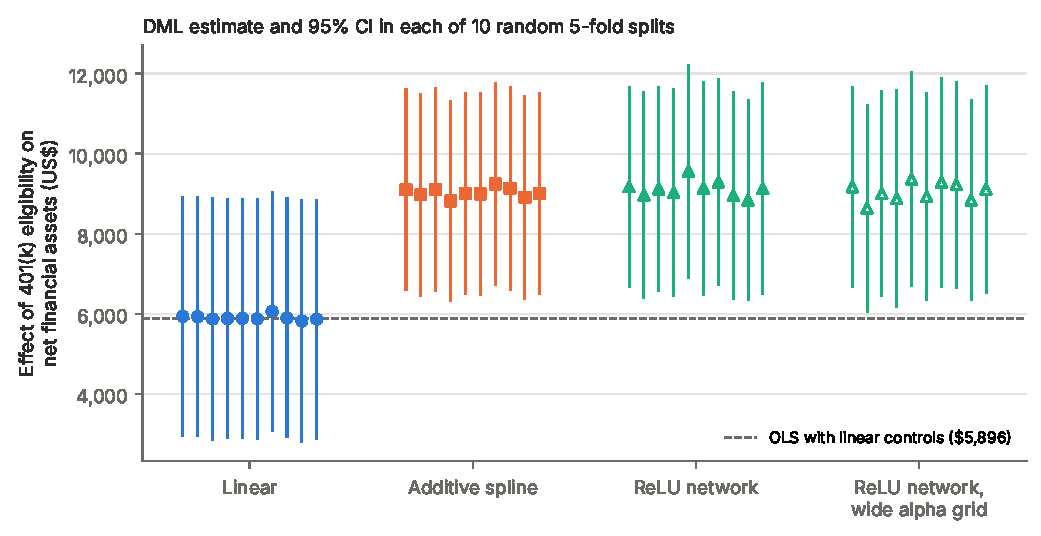
\includegraphics[width=\textwidth]{fig7_401k.pdf}
\caption{Estimate and 95\% interval for each learner in each of the 10 random splits. The dashed line is OLS with linear controls.}\label{fig:401k}
\end{figure}

Four results stand out (Table~\ref{tab:401k}, Figure~\ref{fig:401k}).
\begin{enumerate}
\item \textbf{Confounding is large.} The raw difference in means, \$19,559, falls to \$5,900--\$9,100 once the controls are partialled out. Eligible households have higher incomes and more education, and these also raise their assets.
\item \textbf{The flexible learners agree.} The spline and the network differ by \$120, less than a tenth of a standard error. Both fit better out of fold than linear regression: $R^2$ of 0.264 and 0.276 for $Y$ against 0.226, and 0.157 and 0.158 for $D$ against 0.139. Their estimates are close to the partially linear estimates of about \$9,000 that \citet{chernozhukov2018} report for the same data.
\item \textbf{Sample splitting barely matters.} Across the 10 splits the estimates vary by a standard deviation of \$64 to \$226, at most 0.17 standard errors.
\item \textbf{The network's penalty does not matter.} With the simulation grid, inner cross-validation picked the smallest value, $\alpha=1$, in 41 of 50 folds for the treatment equation, the edge of the grid. Widening the grid to $\{0.1,\dots,1000\}$ spreads the choices over 0.1 to 3 but moves the estimate only from \$9,122 to \$9,054 and leaves the out-of-fold fit unchanged.
\end{enumerate}

\subsection{Why linear regression gives a smaller effect}

Linear regression lies about \$3,100--\$3,200 below the flexible learners, roughly 2.4 standard errors. The true nuisance functions are unknown, so the decomposition of Section~\ref{sec:decomp} is applied with a flexible learner's fit in place of the truth. On the first split, with $a=\hat m_{\mathrm{ref}}-\hat m_{\mathrm{lin}}$ and $b=\hat\ell_{\mathrm{ref}}-\hat\ell_{\mathrm{lin}}$, the identity gives $\hat\theta_{\mathrm{lin}}-\hat\theta_{\mathrm{ref}}=\text{cross terms}+\En[a(b-\hat\theta_{\mathrm{ref}}a)]/\hat J_{\mathrm{lin}}$ exactly; the reference learner's own score term is zero by construction.

\begin{table}[t]
\centering\small
\caption{Decomposition of the gap between linear regression and a flexible reference learner, split 1 (US\$).}\label{tab:diag}
\begin{tabular}{lrr}
\toprule
Component & Reference = spline & Reference = network\\
\midrule
Cross terms & $-211$ & $-1{,}137$\\
Second-order term & $-2{,}943$ & $-2{,}092$\\
Total $=\hat\theta_{\mathrm{lin}}-\hat\theta_{\mathrm{ref}}$ & $-3{,}154$ & $-3{,}229$\\
$\mathrm{Corr}(a,\hat g_{\mathrm{ref}}-\hat g_{\mathrm{lin}})$ & $-0.69$ & $-0.45$\\
\bottomrule
\end{tabular}
\end{table}

\begin{figure}[t]
\centering
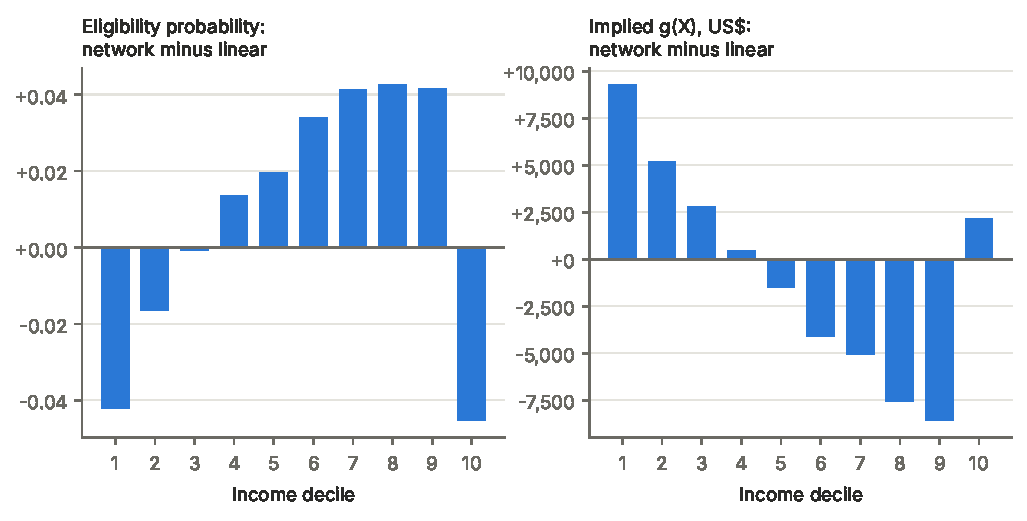
\includegraphics[width=0.92\textwidth]{fig8_401k_misfit.pdf}
\caption{Mean misfit of linear regression relative to the network by income decile, split 1: eligibility probability (left) and implied $g(X)$ (right).}\label{fig:misfit}
\end{figure}

The second-order term accounts for 93\% of the gap against the spline and 65\% against the network (Table~\ref{tab:diag}). As in DGP~A, the two misfits are aligned. Figure~\ref{fig:misfit} shows where: for households in the fourth to ninth income deciles, linear regression under-predicts the probability of eligibility (by up to 0.04) and over-predicts the assets they would hold without eligibility (by up to \$8,600). Its residualised treatment therefore still contains part of the income gradient that its residualised outcome lacks, and the product of the two errors pulls its estimate down. Eligibility and assets both rise with income in a non-linear way that a single linear income term cannot follow.

\subsection{Interpretation}

The application cannot test coverage, because the true effect is unknown, and it rests on conditional exogeneity of eligibility. Within those limits it supports the Monte Carlo conclusions. The learners whose structure can follow the income non-linearity agree with each other and fit better, while the linear learner disagrees in the direction its aligned misfit predicts. By the principles of Section~\ref{sec:guidance}, the estimate of about \$9,000 (95\% interval roughly \$6,500 to \$11,700) is the more credible one. Code: \code{application\_401k.py} and \code{app401k\_diagnostic.py}.

% =====================================================================
\section{Discussion}\label{sec:disc}

The results reduce the question ``which learner should I use for DML?'' to a narrower one: does the learner's model class contain the nuisance functions closely enough, at this sample size, that the error left over is mostly noise rather than systematic misfit?

\subsection{Approximation error and estimation error play different roles}

A learner's first-stage error has two parts. \textbf{Approximation error} is the distance from the true function to the best function in the learner's class. \textbf{Estimation error} comes from fitting that class to finite data. They affect DML in opposite ways.
\begin{itemize}
\item Approximation error is systematic. When $\hat m$ and $\hat g$ both miss the same feature ($X_2^2$ for linear regression in DGP~A, $X_1X_2$ for the spline in DGP~B), the two errors are aligned and their product has a large mean. It does not shrink with $n$.
\item Estimation error is largely noise. The errors in $\hat m$ and $\hat g$ are only weakly related, so their product averages towards zero. This is why the spline in DGP~A at $p=50$ has a large test-sample error but a small bias.
\end{itemize}
The upper-bound proxy $\Rnuis$ cannot tell these apart, because it multiplies norms and ignores direction. The exact second-order term can, and it predicts coverage almost perfectly. For simulation studies of DML, the second-order term is the more informative diagnostic; $\Rnuis$ remains useful as a conservative warning.

\subsection{\texorpdfstring{Why coverage can fall as $n$ grows}{Why coverage can fall as n grows}}

With a fixed approximation error the bias is constant, while the standard error falls like $n^{-1/2}$. The standardised bias, and with it the coverage failure, therefore grows like $\sqrt n$. This is not a finite-sample anomaly: it is what condition \eqref{eq:rate} predicts when a learner's error does not go to zero. In practice it means that a large sample is no protection against a poorly matched learner. A narrow interval from a large sample may simply be a precise estimate of the wrong number.

\subsection{The network's advantage is conditional}

H3 holds only when the network has enough data relative to the number of covariates. At $n=2000$, $p=10$ in DGP~B its error for $\ell$ (0.40) is the only one below the additive floor and its coverage is 0.88. With $p=50$, or with $n=500$, it does no better than the spline. In DGP~A it is clearly beaten by the spline, which supports H2. Two features of the network explain this. Its L2 penalty shrinks all weights equally and cannot discard irrelevant inputs. And at $n=500$ the inner cross-validation that chooses the penalty works on roughly 200 observations per fold and picks noisy values (Appendix~\ref{app:alpha}). Flexibility helps only when the data can pin down the extra structure.

\subsection{Cross-fitting}

Section~\ref{sec:robust} shows that, for this heavily regularised network, dropping cross-fitting did not raise the bias. Instead the cross terms, which are zero on average with cross-fitting, became negative and partly offset the second-order term. This is a coincidence of sign rather than a benefit; a learner that overfits more, or a design in which the two terms share a sign, would show the classic overfitting bias. The robust lesson is that without sample splitting the decomposition loses its clean structure. The estimate then depends on a term that theory gives no control over, and at $n=500$ the standard error understated the spread of the estimates.

\subsection{Practical guidance}\label{sec:guidance}

For applied work with DML, the results suggest five habits.
\begin{enumerate}
\item Report the out-of-fold fit of each nuisance model, not just $\hat\theta$ and its standard error.
\item Estimate with several learners whose model classes differ (additive, interactive, linear). Agreement across them is evidence that the second-order term is small; disagreement points to a misfit in at least one.
\item Prefer a learner whose structure matches what is known about the problem. A flexible learner is not automatically safer when the data are limited.
\item Do not read stability of $\hat\theta$ as $n$ grows as validation. A misspecified learner gives stable, precise and biased estimates.
\item When a simulation calibrated to the application is feasible, compute the second-order term directly.
\end{enumerate}

\subsection{Limitations}

The evidence is finite-sample and specific to this design.
\begin{itemize}
\item The results use $R=50$ replications. Coverage near 0.5 carries a Monte Carlo standard error of about 0.07; the planned main run with $R=300$ will reduce it to about 0.03.
\item Only the partially linear model, two DGPs with Gaussian covariates and homoskedastic Gaussian errors, and two values each of $n$ and $p$ are studied.
\item The network is small, its learning rate is fixed, and its penalty grid was chosen after a preliminary check. A larger architecture, other regularisers or more careful tuning could change its ranking.
\item The cross and oracle terms of decomposition \eqref{eq:decomp} were recorded for 30 of the 50 replications in each cell.
\item The empirical application in Section~\ref{sec:app} cannot test coverage, relies on conditional exogeneity of eligibility, and its diagnostic uses a flexible learner's fit in place of the unknown truth.
\end{itemize}

% =====================================================================
\section{Conclusion}\label{sec:concl}

In this experiment, the coverage of DML confidence intervals is explained by one quantity: the second-order term of the orthogonal score, the product of the errors in $\hat m$ and in the implied $\hat g$. That term is large when the learner's model class misses a feature of the true functions that appears in both, and small when the leftover error is mostly noise. Structural match therefore matters more than the learner's name or its flexibility. The four hypotheses fare as follows.

\begin{table}[h]
\centering\small
\caption*{Verdicts on the hypotheses.}
\begin{tabularx}{\textwidth}{>{\raggedright\arraybackslash}p{4.1cm}>{\raggedright\arraybackslash}p{2.6cm}>{\raggedright\arraybackslash}X}
\toprule
Hypothesis & Verdict & Evidence\\
\midrule
H1: larger remainder, lower coverage & Supported & Bias and second-order term correlate at 0.998; coverage predicted from that term alone is within 0.03 of the observed rate on average\\
H2: in the additive design, splines no worse than the network & Supported & Spline errors are lowest in every DGP~A cell; coverage 0.88--0.92 in three of four cells (0.28 at $n=500$, $p=50$), against 0.02--0.64 for the network\\
H3: in the interactive design, the network better & Partly supported & Only at $n=2000$, $p=10$ (coverage 0.88 against 0.14 for the spline); no advantage at $n=500$ or $p=50$\\
H4: cross-fitting reduces bias or stabilises coverage & Not supported for bias; some support for stability & Without cross-fitting, bias fell (0.021 to 0.006 at $n=2000$) through offsetting cross terms; at $n=500$ the SE understated the spread (SE/sd 0.83)\\
\bottomrule
\end{tabularx}
\end{table}

Two lessons extend beyond this design. First, the exact second-order term is a far better diagnostic of coverage than the usual upper-bound proxy, because the proxy cannot tell systematic misfit from noise. Second, a learner whose error stalls at its approximation limit gives intervals that get worse as the sample grows. A large sample does not protect against a poorly matched first stage.

The 401(k) application points the same way: the two flexible learners agree on about \$9,000, and linear regression's lower estimate is explained by an aligned income misfit. Two extensions follow directly from the code as it stands: the main run with 300 replications per cell, and designs with heteroskedastic errors or a random forest as a fourth learner.

% =====================================================================
\begin{thebibliography}{99}\setlength{\itemsep}{2pt}

\bibitem[Bach et~al.(2022)]{bach2022} Bach, P., Chernozhukov, V., Kurz, M.~S., and Spindler, M. (2022). DoubleML: An object-oriented implementation of double machine learning in Python. \emph{Journal of Machine Learning Research}, 23(53), 1--6.

\bibitem[Bach et~al.(2024)]{bach2024} Bach, P., Kurz, M.~S., Chernozhukov, V., Spindler, M., and Klaassen, S. (2024). DoubleML: An object-oriented implementation of double machine learning in R. \emph{Journal of Statistical Software}, 108(3), 1--56.

\bibitem[Belloni et~al.(2014)]{belloni2014} Belloni, A., Chernozhukov, V., and Hansen, C. (2014). Inference on treatment effects after selection among high-dimensional controls. \emph{Review of Economic Studies}, 81(2), 608--650.

\bibitem[Chen and Parker(2014)]{chen2014} Chen, T. and Parker, T. (2014). Semiparametric efficiency for partially linear single-index regression models. \emph{Journal of Multivariate Analysis}, 130, 376--386.

\bibitem[Chernozhukov et~al.(2018)]{chernozhukov2018} Chernozhukov, V., Chetverikov, D., Demirer, M., Duflo, E., Hansen, C., Newey, W., and Robins, J. (2018). Double/debiased machine learning for treatment and structural parameters. \emph{The Econometrics Journal}, 21(1), C1--C68.

\bibitem[Farrell et~al.(2021)]{farrell2021} Farrell, M.~H., Liang, T., and Misra, S. (2021). Deep neural networks for estimation and inference. \emph{Econometrica}, 89(1), 181--213.

\bibitem[Hastie and Tibshirani(1990)]{hastie1990} Hastie, T. and Tibshirani, R. (1990). \emph{Generalized Additive Models}. London: Chapman and Hall.

\bibitem[Newey(1994)]{newey1994} Newey, W.~K. (1994). The asymptotic variance of semiparametric estimators. \emph{Econometrica}, 62(6), 1349--1382.

\bibitem[Neyman(1959)]{neyman1959} Neyman, J. (1959). Optimal asymptotic tests of composite statistical hypotheses. In U.~Grenander (Ed.), \emph{Probability and Statistics: The Harald Cram\'er Volume}, 213--234. Stockholm: Almqvist and Wiksell.

\bibitem[Pedregosa et~al.(2011)]{pedregosa2011} Pedregosa, F., Varoquaux, G., Gramfort, A., et~al. (2011). Scikit-learn: Machine learning in Python. \emph{Journal of Machine Learning Research}, 12, 2825--2830.

\bibitem[Robinson(1988)]{robinson1988} Robinson, P.~M. (1988). Root-N-consistent semiparametric regression. \emph{Econometrica}, 56(4), 931--954.

\bibitem[Schmidt-Hieber(2020)]{schmidthieber2020} Schmidt-Hieber, J. (2020). Nonparametric regression using deep neural networks with ReLU activation function. \emph{The Annals of Statistics}, 48(4), 1875--1897.

\bibitem[Stone(1982)]{stone1982} Stone, C.~J. (1982). Optimal global rates of convergence for nonparametric regression. \emph{The Annals of Statistics}, 10(4), 1040--1053.

\bibitem[Stone(1985)]{stone1985} Stone, C.~J. (1985). Additive regression and other nonparametric models. \emph{The Annals of Statistics}, 13(2), 689--705.

\end{thebibliography}

% =====================================================================
\appendix
\renewcommand{\thetable}{\Alph{section}\arabic{table}}
\makeatletter\@addtoreset{table}{section}\makeatother

\section{Checks on the data generating processes}\label{app:dgp}

Before any learner was run, the DGP code passed four groups of checks (\code{check\_dgp.py}):
\begin{enumerate}
\item Reproducibility: the same seed returns the same sample.
\item Model identities: $D=m_0+V$, $Y=\theta_0D+g_0+U$ and $Y-\ell_0=\theta_0V+U$ hold exactly.
\item Irrelevance: replacing $X_5$ to $X_p$ with fresh draws leaves $m_0$ and $g_0$ unchanged.
\item Moments: on 400,000 draws the sample covariance of $X$ matches $\Sigma$ to within 0.01 and $\E[X_2^2-1]$ is within 0.01 of zero.
\end{enumerate}
The oracle estimator, which uses the true $\ell_0$ and $m_0$, was then run 1,000 times per design to check the normal approximation and the standard-error formula with no first-stage error (Table~\ref{tab:oracle}). Coverage is within Monte Carlo error ($\pm0.014$) of 0.95 in all four designs, so any coverage shortfall in Section~\ref{sec:results} is due to first-stage error.

\begin{table}[h]
\centering\small
\caption{Oracle DML with true nuisance functions, $p=10$, $R=1{,}000$.}\label{tab:oracle}
\begin{tabular}{ccrrrr}
\toprule
DGP & $n$ & Bias & $\mathrm{sd}(\hat\theta)$ & Mean SE & Coverage\\
\midrule
A & 500 & $-0.001$ & 0.047 & 0.044 & 0.941\\
A & 2000 & 0.000 & 0.023 & 0.022 & 0.944\\
B & 500 & $-0.001$ & 0.044 & 0.045 & 0.948\\
B & 2000 & 0.001 & 0.023 & 0.022 & 0.947\\
\bottomrule
\end{tabular}
\end{table}

\section{Choice of the network's L2 penalty}\label{app:alpha}

The network was fitted with fixed $\alpha$ values from 0.1 to 1,000 on three samples per design. Test-sample error was computed against the true functions, at training sizes equal to four-fifths of $n$ (Table~\ref{tab:alpha}).

\begin{table}[h]
\centering\small
\caption{Best fixed $\alpha$ and test-sample $L_2$ error of the network. The last column is the error of predicting the mean, $\mathrm{sd}(f)$.}\label{tab:alpha}
\begin{tabular}{cccccrrrr}
\toprule
DGP & $n$ & $p$ & Target & Best $\alpha$ & Error at best & Error at $\alpha=1$ & Error at $\alpha=100$ & $\mathrm{sd}(f)$\\
\midrule
A & 500 & 10 & $\ell$ & 3 & 0.680 & 0.756 & 1.382 & 1.513\\
A & 500 & 10 & $m$ & 10 & 0.328 & 0.411 & 0.576 & 0.616\\
A & 500 & 50 & $\ell$ & 10 & 0.960 & 1.273 & 1.465 & 1.505\\
A & 500 & 50 & $m$ & 30 & 0.464 & 0.638 & 0.607 & 0.613\\
A & 2000 & 10 & $\ell$ & 3 & 0.413 & 0.434 & 1.353 & 1.513\\
A & 2000 & 10 & $m$ & 3 & 0.271 & 0.304 & 0.567 & 0.616\\
A & 2000 & 50 & $\ell$ & 10 & 0.619 & 0.868 & 1.450 & 1.505\\
A & 2000 & 50 & $m$ & 10 & 0.359 & 0.504 & 0.596 & 0.613\\
B & 500 & 10 & $\ell$ & 10 & 0.609 & 0.662 & 0.643 & 0.622\\
B & 500 & 10 & $m$ & 10 & 0.246 & 0.322 & 0.302 & 0.307\\
B & 500 & 50 & $\ell$ & 300 & 0.630 & 0.821 & 0.631 & 0.622\\
B & 500 & 50 & $m$ & 30 & 0.309 & 0.489 & 0.313 & 0.305\\
B & 2000 & 10 & $\ell$ & 3 & 0.413 & 0.484 & 0.629 & 0.622\\
B & 2000 & 10 & $m$ & 3 & 0.232 & 0.259 & 0.307 & 0.307\\
B & 2000 & 50 & $\ell$ & 10 & 0.621 & 0.701 & 0.627 & 0.622\\
B & 2000 & 50 & $m$ & 10 & 0.291 & 0.387 & 0.314 & 0.305\\
\bottomrule
\end{tabular}
\end{table}

The optimum lies between 3 and 30 in 15 of 16 cases; more data calls for a smaller penalty and more irrelevant covariates for a larger one. In the remaining case (DGP~B, $n=500$, $p=50$, target $\ell$) no value of $\alpha$ beats predicting the mean. Under inner 3-fold cross-validation on fresh samples, a finer grid $\{2,4,8,16,32,64\}$ reduced the average test error by about 1\% relative to the grid used (0.488 against 0.492). This difference is not significant (paired difference $-0.004$, standard error 0.003, 80 comparisons), so the grid was kept.

\begin{landscape}
\section{Full results}\label{app:full}
\begin{center}\scriptsize
\captionof{table}{All grid points and learners, $R=50$. $e_m$ and $e_l$ are median test-sample errors; $\hat R_2/\mathrm{sd}$ is the mean second-order term divided by $\mathrm{sd}(\hat\theta)$; predicted coverage comes from \eqref{eq:cov}.}\label{tab:full}
\setlength{\tabcolsep}{4pt}
\begin{tabular}{cccl rrr rr r r rr r r r}
\toprule
DGP & $n$ & $p$ & Learner & Bias & $\mathrm{sd}(\hat\theta)$ & RMSE & Coverage & MC SE & SE/sd & CI length & $e_m$ & $e_l$ & $\Rnuis$ & $\hat R_2/\mathrm{sd}$ & Pred.\ cov.\\
\midrule
A & 500 & 10 & Oracle & 0.005 & 0.040 & 0.040 & 0.98 & 0.020 & 1.13 & 0.177 &  &  &  & 0.00 & 0.97\\
A & 500 & 10 & Linear & 0.262 & 0.052 & 0.267 & 0.00 & 0.000 & 1.15 & 0.235 & 0.415 & 0.969 & 13.0 & 4.94 & 0.00\\
A & 500 & 10 & Spline & 0.027 & 0.049 & 0.055 & 0.90 & 0.042 & 0.98 & 0.187 & 0.320 & 0.446 & 5.5 & 0.43 & 0.92\\
A & 500 & 10 & Network & 0.082 & 0.053 & 0.097 & 0.60 & 0.069 & 0.95 & 0.195 & 0.418 & 0.664 & 10.4 & 1.45 & 0.66\\
A & 500 & 50 & Oracle & $-0.005$ & 0.042 & 0.041 & 0.96 & 0.028 & 1.08 & 0.175 &  &  &  & 0.00 & 0.97\\
A & 500 & 50 & Linear & 0.233 & 0.060 & 0.241 & 0.02 & 0.020 & 0.95 & 0.222 & 0.559 & 1.087 & 20.5 & 4.14 & 0.01\\
A & 500 & 50 & Spline & 0.117 & 0.058 & 0.130 & 0.28 & 0.063 & 0.91 & 0.206 & 0.472 & 0.847 & 13.9 & 2.29 & 0.30\\
A & 500 & 50 & Network & 0.224 & 0.062 & 0.232 & 0.02 & 0.020 & 0.89 & 0.216 & 0.608 & 1.149 & 24.2 & 3.72 & 0.02\\
A & 2000 & 10 & Oracle & 0.001 & 0.025 & 0.025 & 0.92 & 0.038 & 0.87 & 0.087 &  &  &  & 0.00 & 0.91\\
A & 2000 & 10 & Linear & 0.242 & 0.033 & 0.244 & 0.00 & 0.000 & 0.91 & 0.116 & 0.385 & 0.944 & 22.9 & 7.41 & 0.00\\
A & 2000 & 10 & Spline & 0.005 & 0.025 & 0.026 & 0.92 & 0.038 & 0.88 & 0.088 & 0.176 & 0.229 & 3.3 & 0.10 & 0.91\\
A & 2000 & 10 & Network & 0.038 & 0.028 & 0.047 & 0.64 & 0.068 & 0.83 & 0.091 & 0.227 & 0.399 & 6.4 & 1.27 & 0.64\\
A & 2000 & 50 & Oracle & $-0.002$ & 0.023 & 0.023 & 0.94 & 0.034 & 0.97 & 0.087 &  &  &  & 0.00 & 0.94\\
A & 2000 & 50 & Linear & 0.244 & 0.030 & 0.246 & 0.00 & 0.000 & 0.99 & 0.116 & 0.423 & 0.972 & 26.4 & 8.38 & 0.00\\
A & 2000 & 50 & Spline & 0.004 & 0.026 & 0.026 & 0.88 & 0.046 & 0.89 & 0.091 & 0.344 & 0.467 & 12.4 & 0.35 & 0.90\\
A & 2000 & 50 & Network & 0.095 & 0.026 & 0.098 & 0.02 & 0.020 & 0.94 & 0.097 & 0.356 & 0.630 & 15.8 & 3.83 & 0.02\\
B & 500 & 10 & Oracle & $-0.004$ & 0.040 & 0.039 & 0.98 & 0.020 & 1.12 & 0.173 &  &  &  & 0.00 & 0.97\\
B & 500 & 10 & Linear & 0.084 & 0.048 & 0.096 & 0.56 & 0.070 & 1.01 & 0.189 & 0.303 & 0.659 & 6.7 & 1.85 & 0.55\\
B & 500 & 10 & Spline & 0.070 & 0.046 & 0.083 & 0.72 & 0.063 & 1.05 & 0.189 & 0.277 & 0.612 & 5.6 & 1.63 & 0.67\\
B & 500 & 10 & Network & 0.060 & 0.047 & 0.076 & 0.82 & 0.054 & 1.02 & 0.189 & 0.316 & 0.635 & 6.8 & 1.36 & 0.74\\
B & 500 & 50 & Oracle & $-0.002$ & 0.047 & 0.047 & 0.92 & 0.038 & 0.93 & 0.173 &  &  &  & 0.00 & 0.93\\
B & 500 & 50 & Linear & 0.086 & 0.057 & 0.103 & 0.60 & 0.069 & 0.84 & 0.188 & 0.465 & 0.782 & 13.2 & 1.52 & 0.55\\
B & 500 & 50 & Spline & 0.078 & 0.050 & 0.092 & 0.70 & 0.065 & 0.95 & 0.187 & 0.307 & 0.632 & 6.4 & 1.60 & 0.61\\
B & 500 & 50 & Network & 0.077 & 0.054 & 0.094 & 0.72 & 0.063 & 0.87 & 0.185 & 0.364 & 0.663 & 8.8 & 1.47 & 0.60\\
B & 2000 & 10 & Oracle & 0.005 & 0.019 & 0.019 & 0.98 & 0.020 & 1.19 & 0.087 &  &  &  & 0.00 & 0.98\\
B & 2000 & 10 & Linear & 0.091 & 0.020 & 0.093 & 0.00 & 0.000 & 1.19 & 0.095 & 0.265 & 0.631 & 10.7 & 4.43 & 0.02\\
B & 2000 & 10 & Spline & 0.075 & 0.020 & 0.077 & 0.14 & 0.049 & 1.19 & 0.094 & 0.234 & 0.580 & 8.5 & 3.60 & 0.10\\
B & 2000 & 10 & Network & 0.021 & 0.019 & 0.028 & 0.88 & 0.046 & 1.22 & 0.090 & 0.210 & 0.403 & 5.8 & 0.94 & 0.93\\
B & 2000 & 50 & Oracle & 0.001 & 0.021 & 0.020 & 0.96 & 0.028 & 1.08 & 0.087 &  &  &  & 0.00 & 0.97\\
B & 2000 & 50 & Linear & 0.091 & 0.023 & 0.094 & 0.04 & 0.028 & 1.05 & 0.095 & 0.312 & 0.663 & 13.7 & 3.89 & 0.03\\
B & 2000 & 50 & Spline & 0.074 & 0.024 & 0.077 & 0.16 & 0.052 & 1.01 & 0.095 & 0.277 & 0.609 & 10.9 & 3.07 & 0.14\\
B & 2000 & 50 & Network & 0.079 & 0.023 & 0.082 & 0.12 & 0.046 & 1.07 & 0.095 & 0.284 & 0.628 & 11.7 & 3.48 & 0.08\\
\bottomrule
\end{tabular}
\end{center}
\end{landscape}

\section{Code and reproduction}\label{app:code}

\begin{table}[h]
\centering\small
\caption{Code map.}\label{tab:code}
\begin{tabularx}{\textwidth}{>{\raggedright\arraybackslash}p{2.8cm}>{\raggedright\arraybackslash}p{5.4cm}>{\raggedright\arraybackslash}X}
\toprule
Step & File & Role\\
\midrule
Configuration & \code{config.py} & Seeds, grid, replication counts, learner hyperparameters\\
Data & \code{dgp.py} & DGPs A and B, true $m_0$, $g_0$, $\ell_0$, seed streams\\
Checks & \code{check\_dgp.py} & Appendix~\ref{app:dgp}\\
Learners & \code{learners.py} & Linear, additive spline, ReLU network\\
One replication & \code{run\_simulation.py} & DoubleMLPLR fit, test-sample errors, decomposition \eqref{eq:decomp}\\
Grid run & \code{run\_checkpointed.py}, \code{pilot.py} & All grid points and replications, resumable\\
Robustness & \code{run\_checkpointed.py ablation}, \code{ablation.py} & Section~\ref{sec:robust}\\
Summaries & \code{summarize.py}, \code{tables.py} & Tables~\ref{tab:cov}--\ref{tab:robust} and~\ref{tab:full}\\
Figures & \code{figures.py}, \code{remainder.py}, \code{orthogonality\_demo.py} & Figures~\ref{fig:orth}--\ref{fig:proxies}\\
Walkthrough & \code{walkthrough\_second\_order.py} & Appendix~\ref{app:walk}\\
Application & \code{application\_401k.py}, \code{app401k\_diagnostic.py} & Section~\ref{sec:app}\\
Tuning check & \code{extras/alpha\_curve.py}, \code{extras/cv\_compare.py} & Appendix~\ref{app:alpha}\\
\bottomrule
\end{tabularx}
\end{table}

To reproduce, run \code{python check\_dgp.py}, then \code{python run\_checkpointed.py main 1 50} followed by \code{python run\_checkpointed.py merge main outputs/main\_raw.csv}, then the summary and figure scripts on \code{outputs/main\_raw.csv}. For the planned main experiment, replace 50 by 300.

\section{One replication computed step by step}\label{app:walk}

This appendix recomputes one replication by hand, without using DoubleML for any number, and shows that every quantity in Sections~\ref{sec:model} and~\ref{sec:results} is reproduced exactly. The main example is replication 1 of DGP~A with $n=500$, $p=10$ and linear regression (seed 1575613034), a cell where the interval fails. A second example, the additive spline in DGP~A with $n=2000$ and $p=10$, shows a cell where it succeeds. The script \code{walkthrough\_second\_order.py} prints every step for any cell.

\subsection*{E.1 The steps and where they are coded}

\begin{table}[H]
\centering\small
\caption{Steps of one replication, with code location and the value in the main example.}\label{tab:steps}
\begin{tabularx}{\textwidth}{c>{\raggedright\arraybackslash}X>{\raggedright\arraybackslash}p{3.6cm}>{\raggedright\arraybackslash}p{3.8cm}}
\toprule
Step & Computation & Code & Value\\
\midrule
0 & Draw $X,V,U$; set $D=m_0+V$, $Y=\theta_0D+g_0+U$; store $m_0,g_0,\ell_0$ & \code{dgp.simulate} & 500 observations\\
1 & Split into 5 folds & \code{KFold} in \code{run\_one} & 400 training, 100 held out per fold\\
2 & Fit $\ell$ and $m$ on four folds, predict the fifth & \code{learners.py}, \code{DoubleMLPLR.fit} & out-of-fold $\hat\ell(X_i)$, $\hat m(X_i)$\\
3 & Residuals $\tilde D=D-\hat m$, $\tilde Y=Y-\hat\ell$ & inside DoubleML & \\
4 & Solve the orthogonal score; SE and CI & \code{model.coef}, \code{model.se} & $\hat\theta=0.7397$, SE $=0.0666$\\
5 & Check orthogonality on the sample & walkthrough step 5 & slope 0.015 vs.\ 0.317 (naive)\\
6 & Decomposition \eqref{eq:decomp} & \code{score\_decomposition} & second-order term 0.2688\\
7 & Test-sample errors and $\Rnuis$ & end of \code{run\_one} & $e_m=0.427$, $e_l=0.972$, $\Rnuis=13.4$\\
8 & Aggregate the 50 replications & \code{summarize.py} & bias 0.262; predicted and observed coverage 0.00\\
\bottomrule
\end{tabularx}
\end{table}

\subsection*{E.2 Solving the score}

The score is linear in $\theta$, $\psi=\psi_a\theta+\psi_b$ with $\psi_a=-\tilde D^2$ and $\psi_b=\tilde Y\tilde D$. Setting its sample mean to zero:
\[
\hat\theta=\frac{\sum_i\tilde D_i\tilde Y_i}{\sum_i\tilde D_i^2}=\frac{432.640}{584.865}=0.739726,\qquad \hat J=\frac1n\sum_i\tilde D_i^2=1.169731,
\]
\[
\hat\sigma^2=\frac{\frac1n\sum_i\hat\psi_i^2}{\hat J^2}=\frac{3.030501}{1.368270}=2.214841,\qquad \mathrm{SE}=\sqrt{\hat\sigma^2/n}=\sqrt{2.214841/500}=0.066556.
\]
The interval $0.7397\pm1.96\times0.0666=[0.609,0.870]$ does not contain 0.5. DoubleML returns the same estimate and SE (differences $1.1\times10^{-16}$ and $1.4\times10^{-17}$) and the same out-of-fold predictions.

\subsection*{E.3 Orthogonality on this sample}

Take the learner's actual errors as the direction, $\Delta=\hat\eta-\eta_0$, and evaluate the sample mean of each score at $\theta_0$ along $\eta_0+r\Delta$. The naive score is $(Y-\theta D-g(X))D$, moved along $g_0+r\Delta g$ with $\Delta g=\Delta\ell-\theta_0\Delta m$ (Table~\ref{tab:orthnum}).

\begin{table}[H]
\centering\small
\caption{Sample mean of the two scores at $\theta_0$ along $\eta_0+r(\hat\eta-\eta_0)$.}\label{tab:orthnum}
\begin{tabular}{crr}
\toprule
$r$ & Orthogonal score & Naive score\\
\midrule
$-1.0$ & $+0.2512$ & $-0.3671$\\
$-0.5$ & $+0.0227$ & $-0.2087$\\
$0$ & $-0.0486$ & $-0.0504$\\
$+0.5$ & $+0.0373$ & $+0.1080$\\
$+1.0$ & $+0.2804$ & $+0.2664$\\
\bottomrule
\end{tabular}
\end{table}

The orthogonal score is a parabola with slope 0.015 at $r=0$, which is sampling noise of order $n^{-1/2}$; the naive score is a line with slope 0.317. Expression \eqref{eq:path} holds with the coefficients
\[
\En\psi=\underbrace{-0.0486}_{\En[VU]}+r\,\big(\underbrace{0.0038}_{\En[aU]}+\underbrace{0.0108}_{\En[V(b-\theta_0a)]}\big)+r^2\,\underbrace{0.3144}_{\En[a(b-\theta_0a)]},
\]
and at $r=1$ it gives 0.2804, so that $0.2804/1.1697=0.2397=\hat\theta-\theta_0$.

\subsection*{E.4 The decomposition in two replications}

\begin{table}[H]
\centering\footnotesize\setlength{\tabcolsep}{4pt}
\caption{Decomposition \eqref{eq:decomp} in two replications. Each bold number is the raw mean divided by $\hat J$ ($\hat J=1.170$ in the first replication and 1.067 in the second).}\label{tab:twoex}
\begin{tabular}{lll}
\toprule
Quantity & Linear, DGP A, $n=500$ (fails) & Spline, DGP A, $n=2000$ (covers)\\
\midrule
$\En[VU]$, oracle term & $-0.0486$, $\mathbf{-0.0416}$ & $-0.0340$, $\mathbf{-0.0318}$\\
$\En[aU]+\En[V(b-\theta_0a)]$, cross terms & $0.0038+0.0108$, $\mathbf{+0.0125}$ & $-0.0005-0.0027$, $\mathbf{-0.0030}$\\
$\En[a(b-\theta_0a)]$, second-order term & $0.3144$, $\mathbf{+0.2688}$ & $0.0076$, $\mathbf{+0.0071}$\\
Sum of the three terms & $+0.2397$ & $-0.0277$\\
$\hat\theta-\theta_0$ & $+0.2397$ (diff.\ $1.4\times10^{-16}$) & $-0.0277$ (diff.\ $4.5\times10^{-17}$)\\
Cauchy--Schwarz bound & 0.304 & 0.033\\
$\mathrm{Corr}(a,b-\theta_0a)$ & \textbf{0.88} & \textbf{0.21}\\
\bottomrule
\end{tabular}
\end{table}

What separates the two replications is the alignment of the two errors as much as their size (Table~\ref{tab:twoex}). Linear regression misses $X_2^2$ in both $\hat m$ and $\hat g$, so the errors are strongly aligned and the second-order term nearly reaches its bound (0.27 against 0.30). The spline's errors are mostly noise and the second-order term is a fifth of its bound.

\subsection*{E.5 Test-sample errors}

On the 20,000 test points, the five fold models give $e_m=\|\hat m-m_0\|=0.4271$ and $e_l=\|\hat\ell-\ell_0\|=0.9723$, so $\Rnuis=\sqrt{500}\times0.4271\times1.3994=13.37$. The function \code{run\_one} and the stored row of the simulation output give the same values to the last digit.

\subsection*{E.6 From one replication to coverage}

Across the 50 replications of the main example's cell, the bias is 0.2619 and the mean second-order term 0.2578. With $\mathrm{sd}(\hat\theta)=0.0522$ and mean SE $=0.0600$, the standardised bias is 4.94 and formula \eqref{eq:cov} predicts coverage 0.00, as observed. In the spline cell the standardised bias is 0.10, and the predicted coverage of 0.91 compares with an observed 0.92. Figures~\ref{fig:bias} and~\ref{fig:proxies} repeat this calculation for all 24 learner cells.

\end{document}
